\documentclass[conference]{IEEEtran}
\usepackage{hyperref}
\usepackage{graphicx}
\hyphenation{op-tical net-works semi-conduc-tor}
\begin{document}
\title{Text - Summarization using Conceptual Statistical Extraction}


\author{\IEEEauthorblockN{Vivek Patani}
\IEEEauthorblockA{School of Informatics and Computing\\
Indiana University\\
Bloomington, Indiana -- 47405\\
Email: vpatani@umail.iu.edu}
\and
\IEEEauthorblockN{Jinsu Kim}
\IEEEauthorblockA{School of Informatics and Computing\\
Indiana University\\
Bloomington, Indiana -- 47405\\
Email: jk247@umail.iu.edu}}
\graphicspath{ {/home/flipswitch/junkyard/text-summarizer/documentation/} }
\maketitle
\begin{abstract}
There have been increasing number of researches conducted in the domain of text summarization using different types of contexts using different methods. In this paper, we attempt to summarize text with important facts eliminating redundant or irrelevant information using extractive method. In this paper we focus mostly on extracting entities and concepts which occur more commonly and are meaningful. Our approach is a statistical one, wherein we weigh each concept in terms of relations and how frequently they occur.
\end{abstract}
\IEEEpeerreviewmaketitle



\section{Introduction}
With increasing amount of textual information available, it becomes difficult to find and read important text. Thus, text summarization would be very useful in that it produces important and concise summary and help readers to save time without having to read entire text.\\

Summary can be generated by \textbf{extractive} and \textbf{abstractive} methods. Extractive methods create short summary with each words, POS from whole sentences without modification of words. Abstractive summarization is more complex way, which makes new sentences summarize by paraphrasing sentences of source documents.

% no \IEEEPARstart
The paper talks about the selective picking up of entities in the text. We, in this paper weigh \textbf{entities} heavily over other concepts. An entity may be a person or any proper noun or moreover any noun. We along with this also collect the verbs associated to them. However, a deep dive into the subject tells us that not all verbs represent an important concept related to the paragraph, hence the term selective.\\
We divide the approach into \textbf{5} sections:
\begin{itemize}
\item Sentencifying
\item Anaphora Resolution
\item Dependency Parsing
\item Statistical Inference
\item Entity Recognition
\end{itemize}

We also use a lot of other ideas, but this briefly describes a good overview of the subject we are presenting here. Our focus is on English for different languages hold different semantic syntax, such like languages like Japanese and Chinese have unambiguous sentence ending markers.

\subsection{Relevant Works}
These are a few relevant studies \& works we came across:
\begin{itemize}
\item Several studies summarized text with a machine learning approach. Chuang, W. T., \& Yang, J. (2000, July) extracted sentence segments with automatic text summarize of on patent text data. The study used three supervised learning algorithm, C4.5, Bayesian, DistAI, to train and extract important sentence segments, and all of the methods performed well in generating good summary.

\item Other than text summarization that have been widely studied, there are some studies explored web-page summarization. Shen et al. studied web-page classification algorithm on LookSmart Web dictionary, web summarization. Naïve Bayes and Support Vector Machine were used for classification algorithm to build baseline system. The study showed improvement in using the summarization-based classification algorithm and ensemble classifier than in using text-based algorithm.

\item In the Rusu et al. (2009) [5] study, they analyzed text on Reuters newswire article and extracted triplet information in the base of semantic graph. After triplet generation, they used anaphora resolution for entities and semantic normalization and evaluated document with automatic summarization.
\end{itemize}

\section{Approach and Methodology}

\subsection{Sentencifying}
To begin with we approach the data with splitting of the set of text into simple sentences.
We do this to make relations and dependencies much easier and flexible to detect. The idea here is to break the sentence down at periods with a few reservations such as places like \textit{Dr., Mr., St., etc.} 47\% of the articles written in the Wall street journal represent abbreveations\textsuperscript{[2]}. This problem in NLP is also referred to as Sentence Boundary Disambiguation (SBD), which is the science of detection of the begining and the ending of a sentence.

\subsection{Anaphora Resolution}
The problem of Anaphora Resolution is also termed as pronoun resolution. Let us understand this problem with a brief example, Sentence: Tim walks his dog, he does so every single day. Your mind subconciously decodes that in this context he is Tim and not the dog. The computer not so intelligent as you, needs a few instruction. There are two approaches to solve this problem, namely Eliminative Constraints \& Weighing Preferences. The former uses a set of rules which should be obeyed by both the anaphor and referent and latter method weighs each of the eligible referents and picks the one with the highest score\textsuperscript{[3]}.

\subsection{Dependency Parsing}
This is the most important step in summarizing text. Dependency grammar is based on the relationships between words. $A \rightarrow B$, means B is dependent on A or A governs B. Dependency Parser is simply used to realise the predicate, subject and object in a particular context. We can understand a simple selection of dependency by expressing the structure in head -- dependent relation, functional categories and some structural categories. Phrases can also be represented by simply the same way. Here is an example of a sentence provided with their dependencies parsed in \textit{fig 1}.

\begin{figure}[h!]
\centering
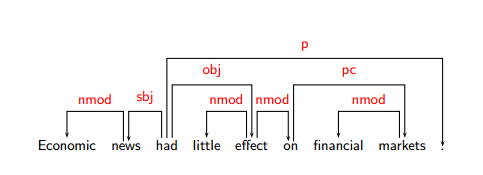
\includegraphics[scale=0.4]{image1}
\caption{Dependency Relation}
    \label{fig:image1}
\end{figure}

\subsection{Statistical Inference}
Once we process the dependencies, we lucidly look for the most important term in all of the text. The term \"most important\" can be interpreted in many ways. For us, we simply pick the term that has occured in most number of concepts (A concept is a tuple of (predicate, subject, object). We pick that term and look for important concepts then and then in those concepts we look for relevant concepts. The advantage of this is that we are looking for the best possible term and finding all the things related to it and pick the best one. The downside is that once a \textit{best term} is picked, only relevant concepts are searched, so our scope is limited to a single \textit{best term} and can cause a single point of failure. We also look for the best predicates, subjects and objects to find out more information in regards to the \textit{best term}.

\subsection{Entity Recognition}
This is the last part and is optional. Named Entity Recognition (NER) is a very interesting property to know for a certain concept or term. It helps us realise whether if the term or concept is a person and often times also helps us realise the gender. This can be helpful in the selection of templates as we can have a customised one for concepts representing people.

\section{Practical Implementation}
We have implemented the above mentioned idea on \href{https://github.com/vivekpatani/text-summarizer}{Github}. You can access the readme and follow the details to run the project.\\
Before you begin, we need to satisfy a few prerequisites, such as:
\begin{itemize}
\item Python 3.5+
\item Java 1.8+
\item MariaDB 10+ (Any MySQL running on default port should do)
\item Docker
\end{itemize}

Let's understand how it works:
\begin{enumerate}
\item Data to be processed in present in a file and the file is read as input (UTF-8) format.
\item Primarily we break down the text into sentences by running it through a sentencer (Stanford NLP provides this).
\item We then take each sentence and run it through a coreref relation generator. This is done to resolve any anaphoras that come across.
\item Once we complete that we take each anaphora and replace each of those with the actual entity.
\item Following that we push it through a Neural Net Depependency Parser (using Stanford NLP). This is the most important step and will cause your quality up or down depending upon how complex sentence structure is.
\item Followed by that we save all the data in a MariaDB database. We store it in a triple store form (predicate, subject, object).
\item We then perform statistical inferences based on the data stored.
\item We find the best term, frequency of each predicate, subject and object and then look for concepts accordingly.
\item Best individual concept and best individual term is giving more prefernce as compared to other things.
\item The best term decides the next step, i.e. Templating.
\item The best term is processed through a Named Entity Recognition Tool.
\item That decides upon what template to pick up and finally that is template we display our best results in.
\end{enumerate}

\section{Conclusion}
The conclusion is that our model that we generated is really focused on a single idea or concept. We focus on one \textit{best term or concept} and use that to find all relevant relations. This is a good idea if the paragraph or text represents exactly one idea, but that is not always the case. The limitations that this implementation holds is, we only focus on a single idea and do not look for any other ideas on it. Sometimes there maybe multiple ideas as important as the previous one and we may still miss it completely revealing an incomplete summary of the text. Also another caveat is that the word disambiguation of different senses may mean different in different contexts, but we do not distinguish that while searching for relevant concepts and hence once again may lead to an incomplete summary.
\section*{Acknowledgment}


We would like to thank our Professor, Dr. Damir Cavar and the teaching assistant, Atreyee Mukherjee for giving us this opportunity and bringing out the best in us.
\begin{thebibliography}{1}

\bibitem{IEEEhowto:kopka}
H.~Kopka and P.~W. Daly, \emph{A Guide to \LaTeX}, 3rd~ed.\hskip 1em plus
  0.5em minus 0.4em\relax Harlow, England: Addison-Wesley, 1999.
\bibitem{}
\href{http://textminingonline.com/dive-into-nltk-part-ii-sentence-tokenize-and-word-tokenize}{Texting Mine Online}
\bibitem{https://nlp.stanford.edu/courses/cs224n/2003/fp/iqsayed/project_report.pdf}
\href{https://nlp.stanford.edu/courses/cs224n/2003/fp/iqsayed/project_report.pdf}{Stanford NLP Text}
\bibitem{}
\href{http://cl.indiana.edu/~md7/13/545/slides/13-dep/13-dep.pdf}{Sandra Kubler and Marcus Dickinson}
\bibitem{}
Chuang, W. T., \& Yang, J. (2000, July). Extracting sentence segments for text summarization: a machine learning approach. In Proceedings of the 23rd annual international ACM SIGIR conference on Research and development in information retrieval (pp. 152-159). ACM.
\bibitem{}
Shen, D., Chen, Z., Yang, Q., Zeng, H. J., Zhang, B., Lu, Y., \& Ma, W. Y. (2004, July). Web-page classification through summarization. In Proceedings of the 27th annual international ACM SIGIR conference on Research and development in information retrieval (pp. 242-249). ACM.
\bibitem{}
Rusu, D., Fortuna, B., Grobelnik, M., \& Mladenic, D. (2009). Semantic Graphs Derived From Triplets with Application in Document Summarization. Informatica (Slovenia), 33(3), 357-362.

\end{thebibliography}
\end{document}